\chapter{Manual de instalación y puesta en marcha de TierraViva}
\label{anexo:manual_instalacion_sistema}

Este anexo describe el procedimiento necesario para instalar y poner en marcha TierraViva a partir del repositorio del proyecto. Su objetivo es permitir que el prototipo pueda reproducirse de forma ordenada, comprobando cada bloque antes de ejecutar una prueba completa.

El manual se centra en la instalación práctica del sistema. Los esquemas eléctricos se recogen en el Anexo~\ref{anexo:esquemas_electricos}; los flujos de funcionamiento, en el Anexo~\ref{anexo:diagramas_flujo_funcionamiento}; la estructura de ThingSpeak, en el Anexo~\ref{anexo:estructura_thingspeak_estados}; y la referencia completa de \textit{endpoints}, en el Anexo~\ref{anexo:manual_api}.

\section{Alcance}

La instalación descrita corresponde a la versión actual de TierraViva, formada por:

\begin{itemize}
    \item una o varias estaciones remotas basadas en Arduino UNO;
    \item publicación de telemetría en ThingSpeak mediante LTE;
    \item Raspberry Pi como nodo local de supervisión;
    \item base de datos SQLite;
    \item API local con FastAPI;
    \item \textit{dashboard} web accesible desde navegador.
\end{itemize}

\section{Requisitos previos}

Antes de comenzar la instalación deben estar disponibles los siguientes elementos:

\begin{itemize}
    \item repositorio del proyecto TierraViva;
    \item Raspberry Pi con Raspberry Pi OS y conexión a Internet;
    \item Arduino IDE para cargar el \textit{firmware} de estación;
    \item cuenta de ThingSpeak;
    \item un canal ThingSpeak por estación;
    \item \texttt{Channel ID}, \texttt{Read API Key} y \texttt{Write API Key} de cada canal;
    \item tarjeta SIM sin PIN activo;
    \item módulo A7670E-LASA con antena conectada;
    \item estación montada según el esquema eléctrico del Anexo~\ref{anexo:esquemas_electricos}.
\end{itemize}

Las claves reales deben mantenerse fuera de la memoria y del repositorio. En la documentación se utilizarán siempre marcadores como \texttt{<READ\_KEY\_A>} o \texttt{<WRITE\_KEY\_A>}.

\section{Preparación de ThingSpeak}

Para cada estación debe existir un canal ThingSpeak independiente. La correspondencia entre campos y variables se encuentra documentada en el Anexo~\ref{anexo:estructura_thingspeak_estados}. Como comprobación mínima, antes de integrar la estación se recomienda verificar que el canal acepta una escritura manual.

\begin{terminaloutput}
https://api.thingspeak.com/update?api_key=<WRITE_KEY>&field1=35
\end{terminaloutput}

Si la petición es correcta, ThingSpeak devuelve un número de entrada. Después debe comprobarse en el canal que se ha registrado una nueva lectura.

\section{Carga del \textit{firmware} de estación}

El \textit{firmware} de la estación se encuentra en:

\begin{terminaloutput}
Estacion/Estacion_A_final_Plus/Estacion_A_final_Plus.ino
\end{terminaloutput}

Antes de cargarlo en Arduino UNO deben revisarse, como mínimo, los siguientes parámetros:

\begin{table}[H]
\centering
\renewcommand{\arraystretch}{1.15}
\rowcolors{2}{TableRowSoft}{white}
\small

\begin{tabular}{|p{0.34\textwidth}|p{0.48\textwidth}|}
\hline
\rowcolor{URJCRed}
\TVHead{Parámetro} & \TVHead{Función} \\
\hline
\texttt{APN} & APN del operador móvil utilizado por la SIM. \\
\hline
\texttt{THINGSPEAK\_API\_KEY} & Clave de escritura del canal ThingSpeak de la estación. \\
\hline
\texttt{SOIL\_DRY} & Valor bruto del sensor en condición seca. \\
\hline
\texttt{SOIL\_WET} & Valor bruto del sensor en condición húmeda. \\
\hline
\texttt{NORMAL\_SOIL\_THRESHOLD} & Umbral de humedad usado en funcionamiento normal. \\
\hline
\texttt{SAFE\_SOIL\_THRESHOLD} & Umbral de humedad usado en modo seguro. \\
\hline
\texttt{IRRIGATION\_SECONDS} & Duración del riego local. \\
\hline
\texttt{COOLDOWN\_MS} & Tiempo mínimo entre dos riegos consecutivos. \\
\hline
\texttt{SEND\_INTERVAL\_MS} & Intervalo de publicación de telemetría. \\
\hline
\end{tabular}
\caption{Parámetros principales que deben revisarse antes de cargar el \textit{firmware}.}
\label{tab:parametros_firmware_instalacion}
\end{table}

\subsection{Librerías empleadas por el \textit{firmware}}
\label{subsec:librerias_firmware_estacion}

El \textit{firmware} de la estación remota utiliza varias librerías de Arduino y de C/C++ para gestionar la comunicación con sensores, el módem LTE y el tratamiento de cadenas. Estas dependencias permiten implementar de forma ordenada los bloques principales del \textit{sketch}: lectura I2C, comunicación serie con el A7670E-LASA, adquisición de medidas ambientales y construcción de peticiones HTTP.

\begin{table}[H]
\centering
\renewcommand{\arraystretch}{1.15}
\rowcolors{2}{TableRowSoft}{white}

\small
\begin{tabular}{|p{0.25\textwidth}|p{0.31\textwidth}|p{0.34\textwidth}|}
\hline
\rowcolor{URJCRed}
\TVHead{Librería} & \TVHead{Uso en TierraViva} & \TVHead{Motivo de utilización} \\
\hline
\texttt{SoftwareSerial} & Comunicación UART entre Arduino UNO y el módem A7670E-LASA mediante los pines \texttt{D10} y \texttt{D11}. & Permite disponer de un puerto serie adicional, manteniendo el puerto serie hardware para programación y depuración por USB. \\
\hline
\texttt{Wire} & Comunicación I2C con los sensores digitales BME280 y BH1750. & Proporciona las funciones necesarias para usar el bus I2C del Arduino UNO, asociado a los pines \texttt{A4/SDA} y \texttt{A5/SCL}. \\
\hline
\texttt{BH1750} & Lectura del sensor de luminosidad BH1750/GY-302. & Permite obtener directamente la iluminancia en lux, evitando trabajar con una lectura analógica sin escala física directa. \\
\hline
\texttt{Adafruit\_Sensor} & Capa común utilizada por sensores de la familia Adafruit. & Proporciona estructuras y tipos comunes requeridos por la librería del BME280. \\
\hline
\texttt{Adafruit\_BME280} & Lectura del sensor ambiental BME280. & Permite obtener temperatura, humedad relativa y presión atmosférica mediante I2C. \\
\hline
\texttt{string.h} & Tratamiento de cadenas en C, como búsqueda de respuestas y construcción de mensajes. & Permite usar funciones como \texttt{strstr()} y \texttt{snprintf()}, útiles para interpretar respuestas del módem y construir peticiones HTTP con buffers controlados. \\
\hline
\end{tabular}
\caption{Librerías principales utilizadas por el \textit{firmware} de estación.}
\label{tab:librerias_firmware_estacion}
\end{table}

El uso de \texttt{SoftwareSerial} requiere una consideración específica. Arduino UNO solo dispone de un puerto serie hardware, utilizado normalmente para cargar el programa y depurar mediante el monitor serie. Por ello, la comunicación con el A7670E-LASA se implementa mediante un puerto serie software en los pines \texttt{D10} y \texttt{D11}. En el montaje de TierraViva, \texttt{D10} recibe datos desde \texttt{TXD} del módem y \texttt{D11} transmite hacia \texttt{RXD} del módem mediante divisor resistivo.

Durante las pruebas se evitó utilizar velocidades elevadas en este puerto serie software. Aunque algunos módems pueden trabajar a baudios superiores, en Arduino UNO \texttt{SoftwareSerial} puede volverse inestable a velocidades altas. Por ese motivo, el \textit{firmware} se estabilizó a \texttt{9600} baudios, priorizando fiabilidad frente a velocidad de transmisión.

Las librerías \texttt{Wire}, \texttt{BH1750} y \texttt{Adafruit\_BME280} permiten integrar los sensores digitales sobre el mismo bus I2C. En la estación, el BH1750 se detectó en la dirección \texttt{0x23} y el BME280 en la dirección \texttt{0x76}, por lo que ambos pueden compartir las líneas \texttt{SDA} y \texttt{SCL} sin conflicto de direcciones.

Por último, \texttt{string.h} se utiliza para trabajar con cadenas de caracteres de forma controlada. Esta decisión es relevante en Arduino UNO porque la memoria SRAM disponible es reducida. Funciones como \texttt{snprintf()} permiten construir cadenas dentro de buffers de tamaño definido, mientras que \texttt{strstr()} permite comprobar si una respuesta del módem contiene textos como \texttt{OK} o códigos HTTP esperados.

La carga del \textit{firmware} se realiza desde Arduino IDE:

\begin{enumerate}
    \item Conectar Arduino UNO al ordenador mediante USB;
    \item Abrir el fichero \texttt{Estacion\_X\_final\_Plus.ino}, siendo \texttt{X} la letra de la estación correspondiente, por ejemplo \texttt{A} o \texttt{B};
    \item Seleccionar la placa \textit{Arduino UNO};
    \item Seleccionar el puerto serie correspondiente;
    \item Comprobar que las librerías indicadas en la Tabla~\ref{tab:librerias_firmware_estacion} están disponibles en el entorno de Arduino;
    \item Compilar el programa;
    \item Cargar el \textit{firmware};
    \item Abrir el monitor serie a \texttt{9600} baudios para comprobar sensores, módem, red LTE y publicación.
\end{enumerate}

La Figura~\ref{fig:arduino_placa_uno} muestra el procedimiento para seleccionar la placa \textit{Arduino UNO} en Arduino IDE. A continuación, la Figura~\ref{fig:arduino_puerto_usb} muestra la selección del puerto serie asociado a la placa conectada por USB.

\begin{figure}[H]
    \centering
    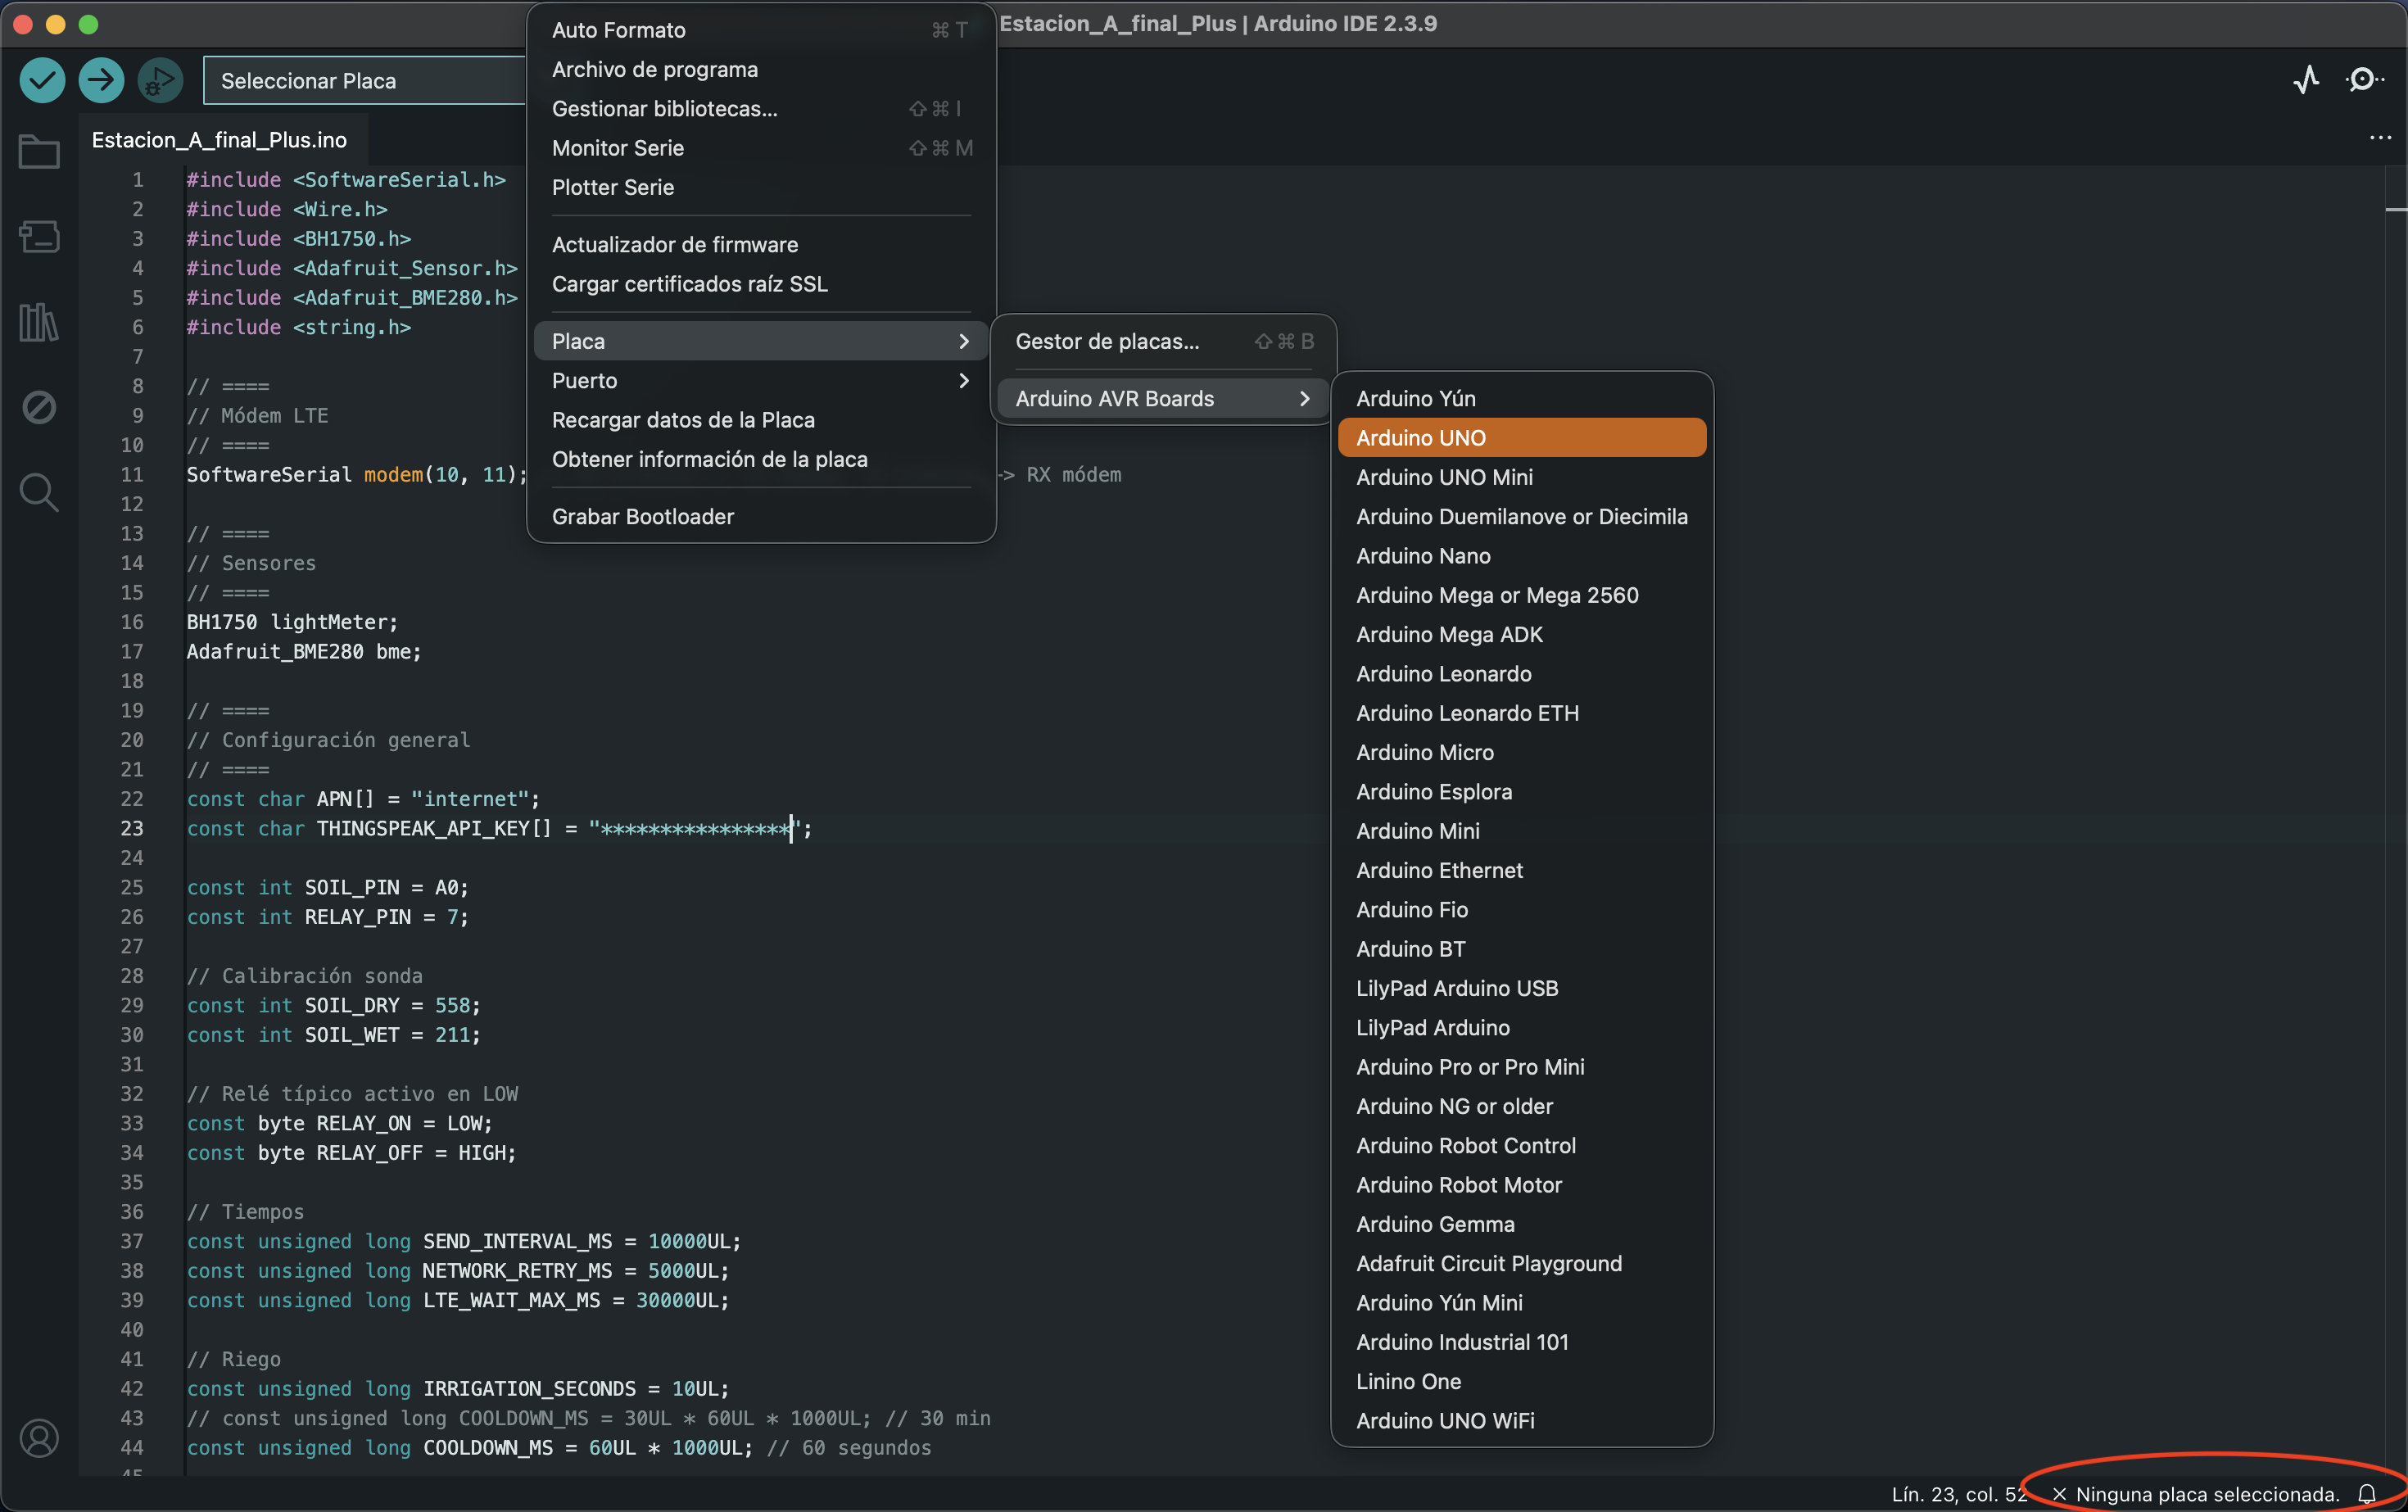
\includegraphics[width=0.92\textwidth]{figs/seleccion_placa_Arduino.png}
    \caption{Selección de la placa \textit{Arduino UNO} en Arduino IDE antes de cargar el \textit{firmware} de la estación. Captura propia.}
    \label{fig:arduino_placa_uno}
\end{figure}

\begin{figure}[H]
    \centering
    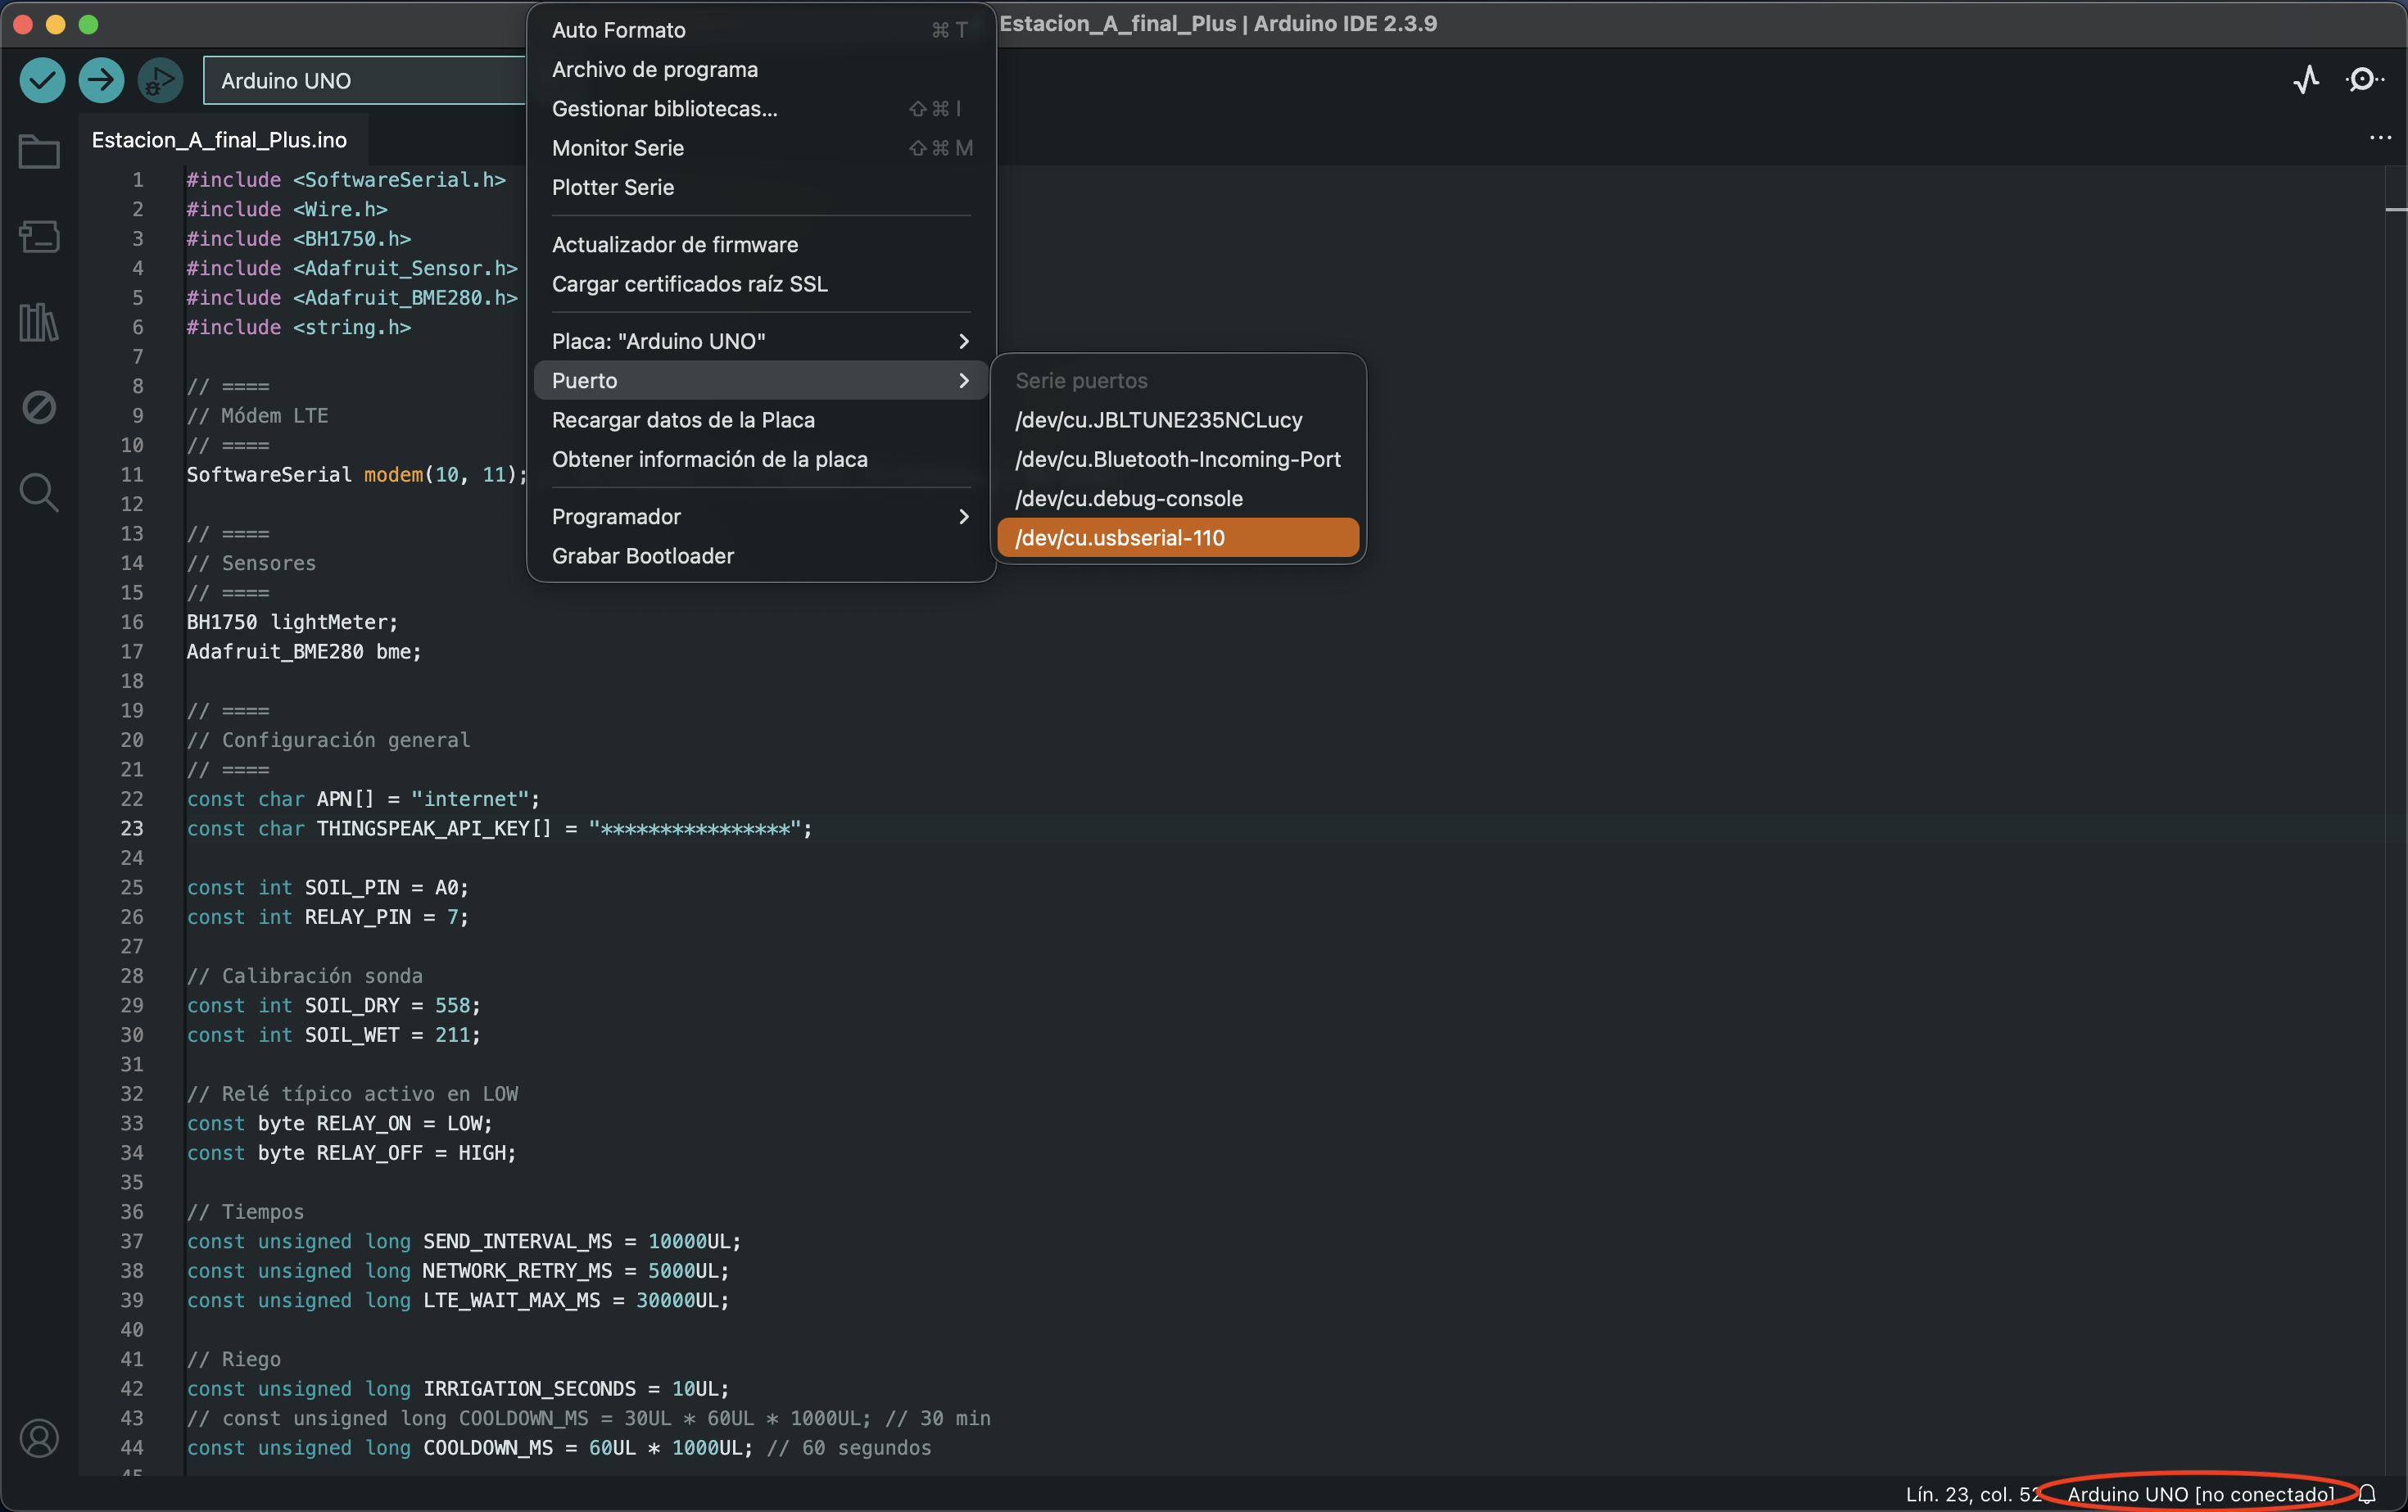
\includegraphics[width=0.92\textwidth]{figs/seleccion_puerto_Arduino.png}
    \caption{Selección del puerto serie correspondiente a la placa Arduino conectada por USB en Arduino IDE. Captura propia.}
    \label{fig:arduino_puerto_usb}
\end{figure}

Debe tenerse en cuenta que el nombre exacto del puerto serie puede variar según el sistema operativo, el adaptador USB empleado y el equipo utilizado durante la instalación.

\section{Instalación del software en Raspberry Pi}

En primer lugar se actualiza el sistema y se instalan las herramientas básicas:

\begin{bashcode}
sudo apt update
sudo apt upgrade -y
sudo apt install -y git python3 python3-venv python3-pip sqlite3
\end{bashcode}

Después se descarga el repositorio:

\begin{bashcode}
cd /home/pi
git clone https://github.com/ltejedorcruz/TierraViva.git
cd TierraViva
\end{bashcode}

Si el repositorio ya existe, puede actualizarse mediante:

\begin{bashcode}
cd /home/pi/TierraViva
git pull
\end{bashcode}

El repositorio incluye un fichero \texttt{requirements.txt} con las dependencias Python necesarias para ejecutar la API y el proceso de ingesta. Durante la instalación, el script \texttt{tierraviva.sh} crea un entorno virtual e instala automáticamente dichas dependencias mediante \texttt{pip}.

\section{Configuración del fichero \texttt{.env}}

El fichero \texttt{.env} debe crearse en la raíz del repositorio. Contiene la configuración local de estaciones, ThingSpeak y parámetros de ejecución.

\begin{bashcode}
nano .env
\end{bashcode}

Un ejemplo de configuración es:

\begin{bashcode}
STATIONS=A,B
STATION_ID=A

THINGSPEAK_CHANNEL_A=<CHANNEL_ID_A>
THINGSPEAK_READ_KEY_A=<READ_KEY_A>

THINGSPEAK_CHANNEL_B=<CHANNEL_ID_B>
THINGSPEAK_READ_KEY_B=<READ_KEY_B>

POLL_INTERVAL_SECONDS=10
REQUEST_TIMEOUT_SECONDS=12

TIERRAVIVA_LOG_LEVEL=INFO
\end{bashcode}

Para facilitar la reproducción del sistema, el repositorio incluye un fichero \texttt{.env.example} con la estructura de variables de entorno requerida. Este fichero no contiene claves reales ni identificadores privados, sino una plantilla que debe copiarse a \texttt{.env} y completarse con los canales y claves de lectura de ThingSpeak correspondientes.

\section{Preparación del \textit{dashboard}}

El \textit{dashboard} fuente se encuentra en el directorio:

\begin{terminaloutput}
dashboard/
\end{terminaloutput}

La interfaz principal se concentra en el fichero:

\begin{terminaloutput}
dashboard/index.html
\end{terminaloutput}

Este fichero incluye la estructura HTML, los estilos CSS embebidos y la lógica JavaScript necesaria para consultar la API y actualizar la interfaz. Los recursos gráficos se almacenan en:

\begin{terminaloutput}
dashboard/images/
\end{terminaloutput}

La API sirve la interfaz desde el directorio de ejecución:

\begin{terminaloutput}
frontend/
\end{terminaloutput}

Durante la instalación, el script \texttt{tierraviva.sh} sincroniza automáticamente el contenido de \texttt{dashboard/} con el directorio \texttt{frontend/}, que es el directorio servido por FastAPI. Esta copia incluye el fichero \texttt{index.html} y los recursos gráficos almacenados en \texttt{dashboard/images/}.

Si se desea realizar esta operación manualmente, o repetirla después de modificar el dashboard, puede ejecutarse:

\begin{bashcode}
mkdir -p frontend
cp -r dashboard/* frontend/
\end{bashcode}

Después de este paso debe existir, al menos:

\begin{terminaloutput}
frontend/index.html
frontend/images/
\end{terminaloutput}

La estructura actual concentra los estilos y la lógica JavaScript en el propio fichero \texttt{index.html}. Esta organización simplifica el despliegue del prototipo, reduce el número de rutas estáticas que deben sincronizarse durante las pruebas y facilita que FastAPI sirva la interfaz desde el directorio \texttt{frontend/}.

\section{Instalación mediante \textit{script}}

Antes de utilizar el \textit{script} debe concederse permiso de ejecución:

\begin{bashcode}
chmod +x tierraviva.sh
\end{bashcode}

La instalación inicial se realiza con:

\begin{bashcode}
./tierraviva.sh install
\end{bashcode}

Este comando prepara el entorno de ejecución del proyecto: crea el entorno virtual, instala dependencias, inicializa la base de datos y crea los directorios necesarios para la ejecución.

Tras la instalación, conviene comprobar que el dashboard se ha sincronizado correctamente con \texttt{frontend/}, especialmente el fichero \texttt{index.html} y el directorio \texttt{images/}:

\begin{bashcode}
ls frontend/
ls frontend/images
\end{bashcode}

La tabla \texttt{readings} almacena lecturas, \texttt{system\_state} conserva información de estado del sistema y \texttt{valve\_events} queda preparada para registrar eventos relacionados con la actuación.

\section{Arranque del sistema}

El sistema se arranca mediante:

\begin{bashcode}
./tierraviva.sh start
\end{bashcode}

Este comando inicia los procesos principales:

\begin{itemize}
    \item \texttt{main.py}, encargado de consultar ThingSpeak y almacenar lecturas nuevas;
    \item \texttt{api.py}, encargado de servir la API y el \textit{dashboard} web.
\end{itemize}

Para detener el sistema se utiliza:

\begin{bashcode}
./tierraviva.sh stop
\end{bashcode}

Para reiniciarlo:

\begin{bashcode}
./tierraviva.sh restart
\end{bashcode}

Para consultar el estado:

\begin{bashcode}
./tierraviva.sh status
\end{bashcode}

Para revisar los \textit{logs}:

\begin{bashcode}
./tierraviva.sh logs
\end{bashcode}

\section{Comprobación de la API}

Con el sistema arrancado, se comprueba primero el estado general de la API:

\begin{bashcode}
curl http://127.0.0.1:8000/api/health
\end{bashcode}

También puede comprobarse desde navegador:

\begin{terminaloutput}
http://<IP_RASPBERRY>:8000/api/health
\end{terminaloutput}

Otras comprobaciones útiles son:

\begin{terminaloutput}
http://<IP_RASPBERRY>:8000/api/config
http://<IP_RASPBERRY>:8000/api/latest?station=A
http://<IP_RASPBERRY>:8000/api/readings?station=A&limit=20
http://<IP_RASPBERRY>:8000/api/stats?station=A&hours=24
\end{terminaloutput}

La descripción completa de \textit{endpoints}, parámetros y respuestas se recoge en el Anexo~\ref{anexo:manual_api}.

\section{Acceso al \textit{dashboard}}

Una vez arrancada la API y copiado el \textit{dashboard} en \texttt{frontend/}, la interfaz web se abre desde:

\begin{terminaloutput}
http://<IP_RASPBERRY>:8000/
\end{terminaloutput}

Si se accede desde la propia Raspberry Pi, puede utilizarse:

\begin{terminaloutput}
http://127.0.0.1:8000/
\end{terminaloutput}

El \textit{dashboard} debe mostrar la estación seleccionada, la última lectura disponible, el estado de frescura, variables ambientales, estado de relé, eventos, gráficas y tabla de lecturas recientes.

\section{Comprobación extremo a extremo}

La instalación se considera preparada cuando se completa la siguiente secuencia:

\begin{table}[H]
\centering
\renewcommand{\arraystretch}{1.15}
\rowcolors{2}{TableRowSoft}{white}

\small
\begin{tabular}{|p{0.38\textwidth}|p{0.42\textwidth}|}
\hline
\rowcolor{URJCRed}
\TVHead{Comprobación} & \TVHead{Resultado esperado} \\
\hline
Estación encendida & Arduino, sensores y módem arrancan de forma estable.\\
\hline
Lectura de sensores & Valores coherentes en el monitor serie.\\
\hline
Registro LTE & El módem registra red móvil.\\
\hline
Publicación en ThingSpeak & Aparece una nueva entrada en el canal.\\
\hline
Ingesta en Raspberry Pi & \texttt{main.py} recupera una lectura nueva.\\
\hline
Inserción en SQLite & La lectura aparece en \texttt{readings}.\\
\hline
API operativa & \texttt{/api/health} responde correctamente.\\
\hline
\textit{Dashboard} visible & La interfaz muestra datos de la estación.\\
\hline
Prueba de relé aislada & El relé conmuta correctamente y vuelve a estado apagado.\\
\hline
Bomba temporizada & La bomba se activa y se apaga tras el tiempo configurado.\\
\hline
\end{tabular}
\caption{Checklist de comprobación extremo a extremo.}
\label{tab:checklist_extremo_a_extremo_instalacion}
\end{table}

\section{Problemas habituales}

\begin{table}[H]
\centering
\renewcommand{\arraystretch}{1.15}
\rowcolors{2}{TableRowSoft}{white}

\scriptsize
\begin{tabular}{|p{0.30\textwidth}|p{0.30\textwidth}|p{0.30\textwidth}|}
\hline
\rowcolor{URJCRed}
\TVHead{Problema} & \TVHead{Causa probable} & \TVHead{Acción recomendada} \\
\hline
Ausencia de datos en ThingSpeak & Clave de escritura incorrecta, APN incorrecto o fallo LTE. & Revisar \textit{firmware}, SIM, antena, APN y monitor serie. \\
\hline
Fallo de recuperación de datos en Raspberry Pi & Canal o clave de lectura incorrectos. & Revisar \texttt{THINGSPEAK\_CHANNEL\_A/B} y \texttt{THINGSPEAK\_READ\_KEY\_A/B}. \\
\hline
Fallo de arranque de la API & Entorno virtual o dependencias pendientes de preparar. & Ejecutar \texttt{./tierraviva.sh install}. \\
\hline
Fallo de carga del \textit{dashboard} & Ausencia de \texttt{frontend/index.html} o sincronización pendiente del contenido de \texttt{dashboard/}. & Ejecutar \texttt{./tierraviva.sh install} o, de forma manual, \texttt{cp -r dashboard/* frontend/}. Comprobar que existen \texttt{frontend/index.html} y \texttt{frontend/images/}. \\
\hline
El \textit{dashboard} carga con recursos gráficos ausentes & Sincronización incompleta del directorio \texttt{images/}. & Repetir \texttt{cp -r dashboard/* frontend/} y revisar que existen los ficheros gráficos en \texttt{frontend/images/}. \\
\hline
Ausencia de registros en SQLite & Publicación pendiente de la estación o ingestor inactivo. & Revisar ThingSpeak y \textit{logs} de \texttt{main.py}. \\
\hline
El relé se activa al arrancar & Lógica invertida o inicialización incorrecta. & Comprobar configuración del \textit{firmware} y probar sin bomba. \\
\hline
Bomba activa fuera del intervalo previsto & Error de cableado o uso del contacto incorrecto del relé. & Usar contacto normalmente abierto y validar apagado por \textit{firmware}. \\
\hline
El módulo LTE se reinicia & Alimentación insuficiente durante transmisión. & Revisar fuente, LM2596, corriente disponible y masa común. \\
\hline
\end{tabular}
\caption{Problemas habituales durante la instalación y puesta en marcha.}
\label{tab:problemas_instalacion_resumido}
\end{table}

\section{Conclusión}

La puesta en marcha de TierraViva debe realizarse por bloques: primero estación y sensores, después publicación en ThingSpeak, más tarde ingesta en Raspberry Pi, base de datos, API, \textit{dashboard} y finalmente actuación sobre relé o bomba. Esta secuencia permite aislar errores, localizar con mayor precisión fallos de montaje, configuración o comunicación, y comprobar cada capa antes de ejecutar una prueba completa.
